% ============================================================
% Paper-ready snippets for the bias / dispersion / MSE study
% (N_int = 160, M = 10^4 pseudo-experiments, backgrounds fluctuated)
%
% Contents:
%   (A) three figure environments  -> paste where Graciela left the slots
%   (B) Appendix D: brief description of the procedure
%
% Figure files to upload to Overleaf (from notes/ensemble/results/paper/):
%   relative_bias_disp_rmse_N160_M10000.pdf
%   abs_b2_s2_mse_N160_M10000.pdf
%   ratio_b2_over_mse_N160_M10000.pdf
%
% Index convention used below: i labels observed recoil-energy bins,
% j labels neutrino-energy intervals, so the bias b_j cannot be confused
% with the background counts b_i.  Adjust \ref/\label names to the paper's.
% ============================================================

% ---------- (A1) relative bias, dispersion, sqrt(MSE) ----------
\begin{figure*}[t]
\centering
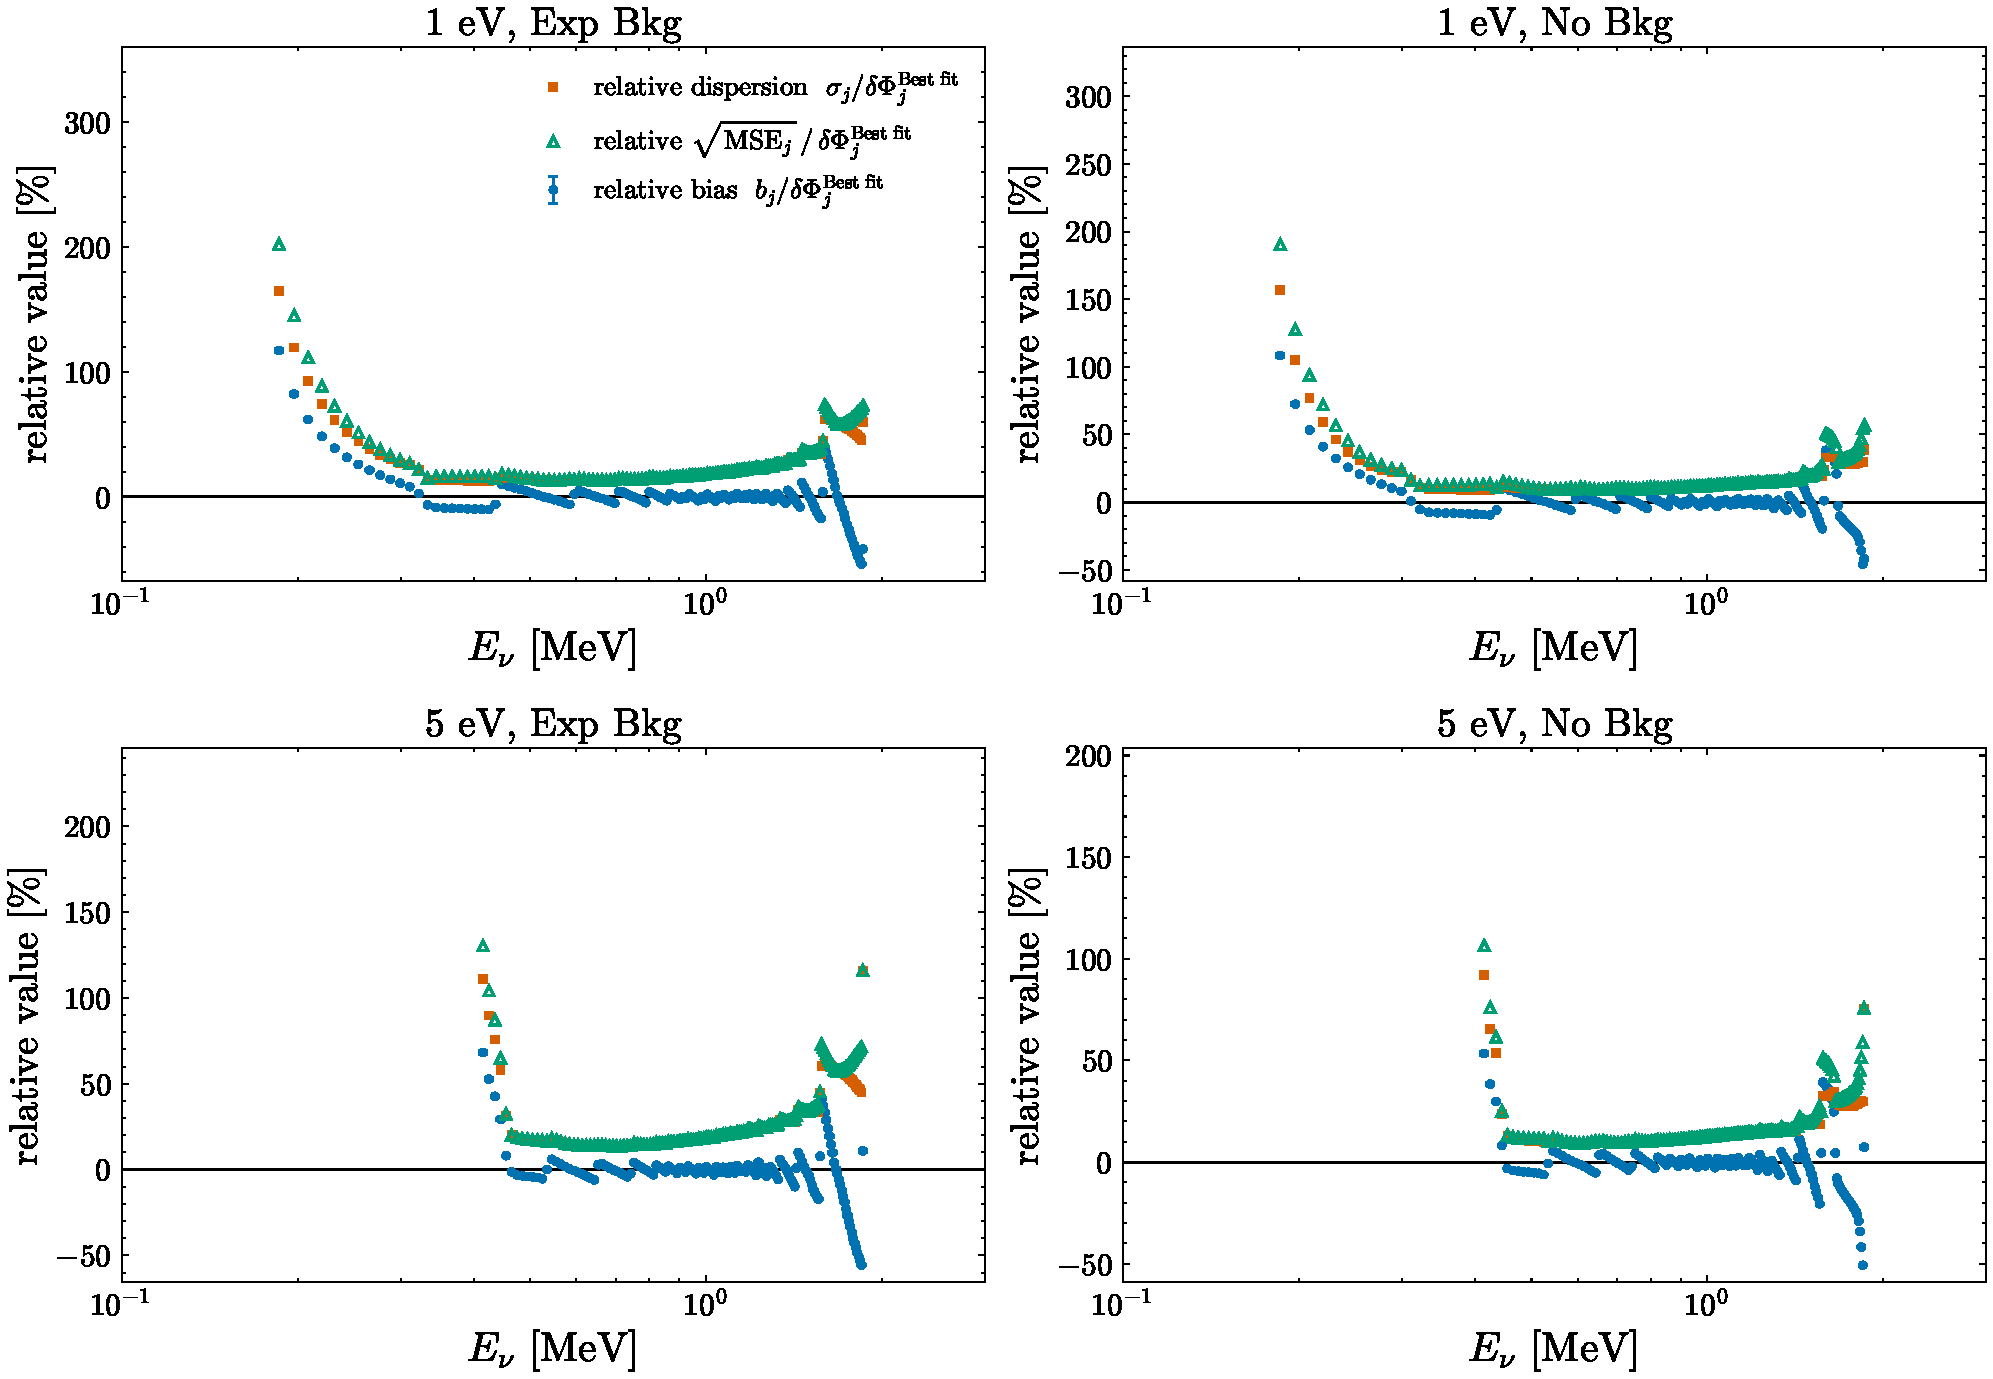
\includegraphics[width=\textwidth]{relative_bias_disp_rmse_N160_M10000.pdf}
\caption{Relative bias $b_j/\delta\Phi_j^{\rm Best\ fit}$ (blue circles),
relative dispersion $\sigma_j/\delta\Phi_j^{\rm Best\ fit}$ (orange squares),
and relative $\sqrt{{\rm MSE}_j}/\delta\Phi_j^{\rm Best\ fit}$ (green open
triangles), with ${\rm MSE}_j=b_j^2+\sigma_j^2$, for the four configurations
considered (1~eV and 5~eV thresholds, with and without background, 3~kg~yr).
All quantities are obtained from $M=10^4$ pseudo-experiments with
$N_{\rm int}=160$ as described in Appendix~\ref{app:biasprocedure}.
The error bars on the bias show its Monte-Carlo uncertainty
$\sigma_j/\sqrt{M}$.  Intervals where $\delta\Phi_j^{\rm Best\ fit}=0$
(at the highest energies) are omitted.  The bias is well below the
dispersion except in the lowest- and highest-energy intervals, so
$\sqrt{{\rm MSE}_j}$ essentially coincides with $\sigma_j$ over most of
the energy range.}
\label{fig:relbiasdisp}
\end{figure*}

% ---------- (A2) b^2, sigma^2, MSE in absolute units ----------
\begin{figure*}[t]
\centering
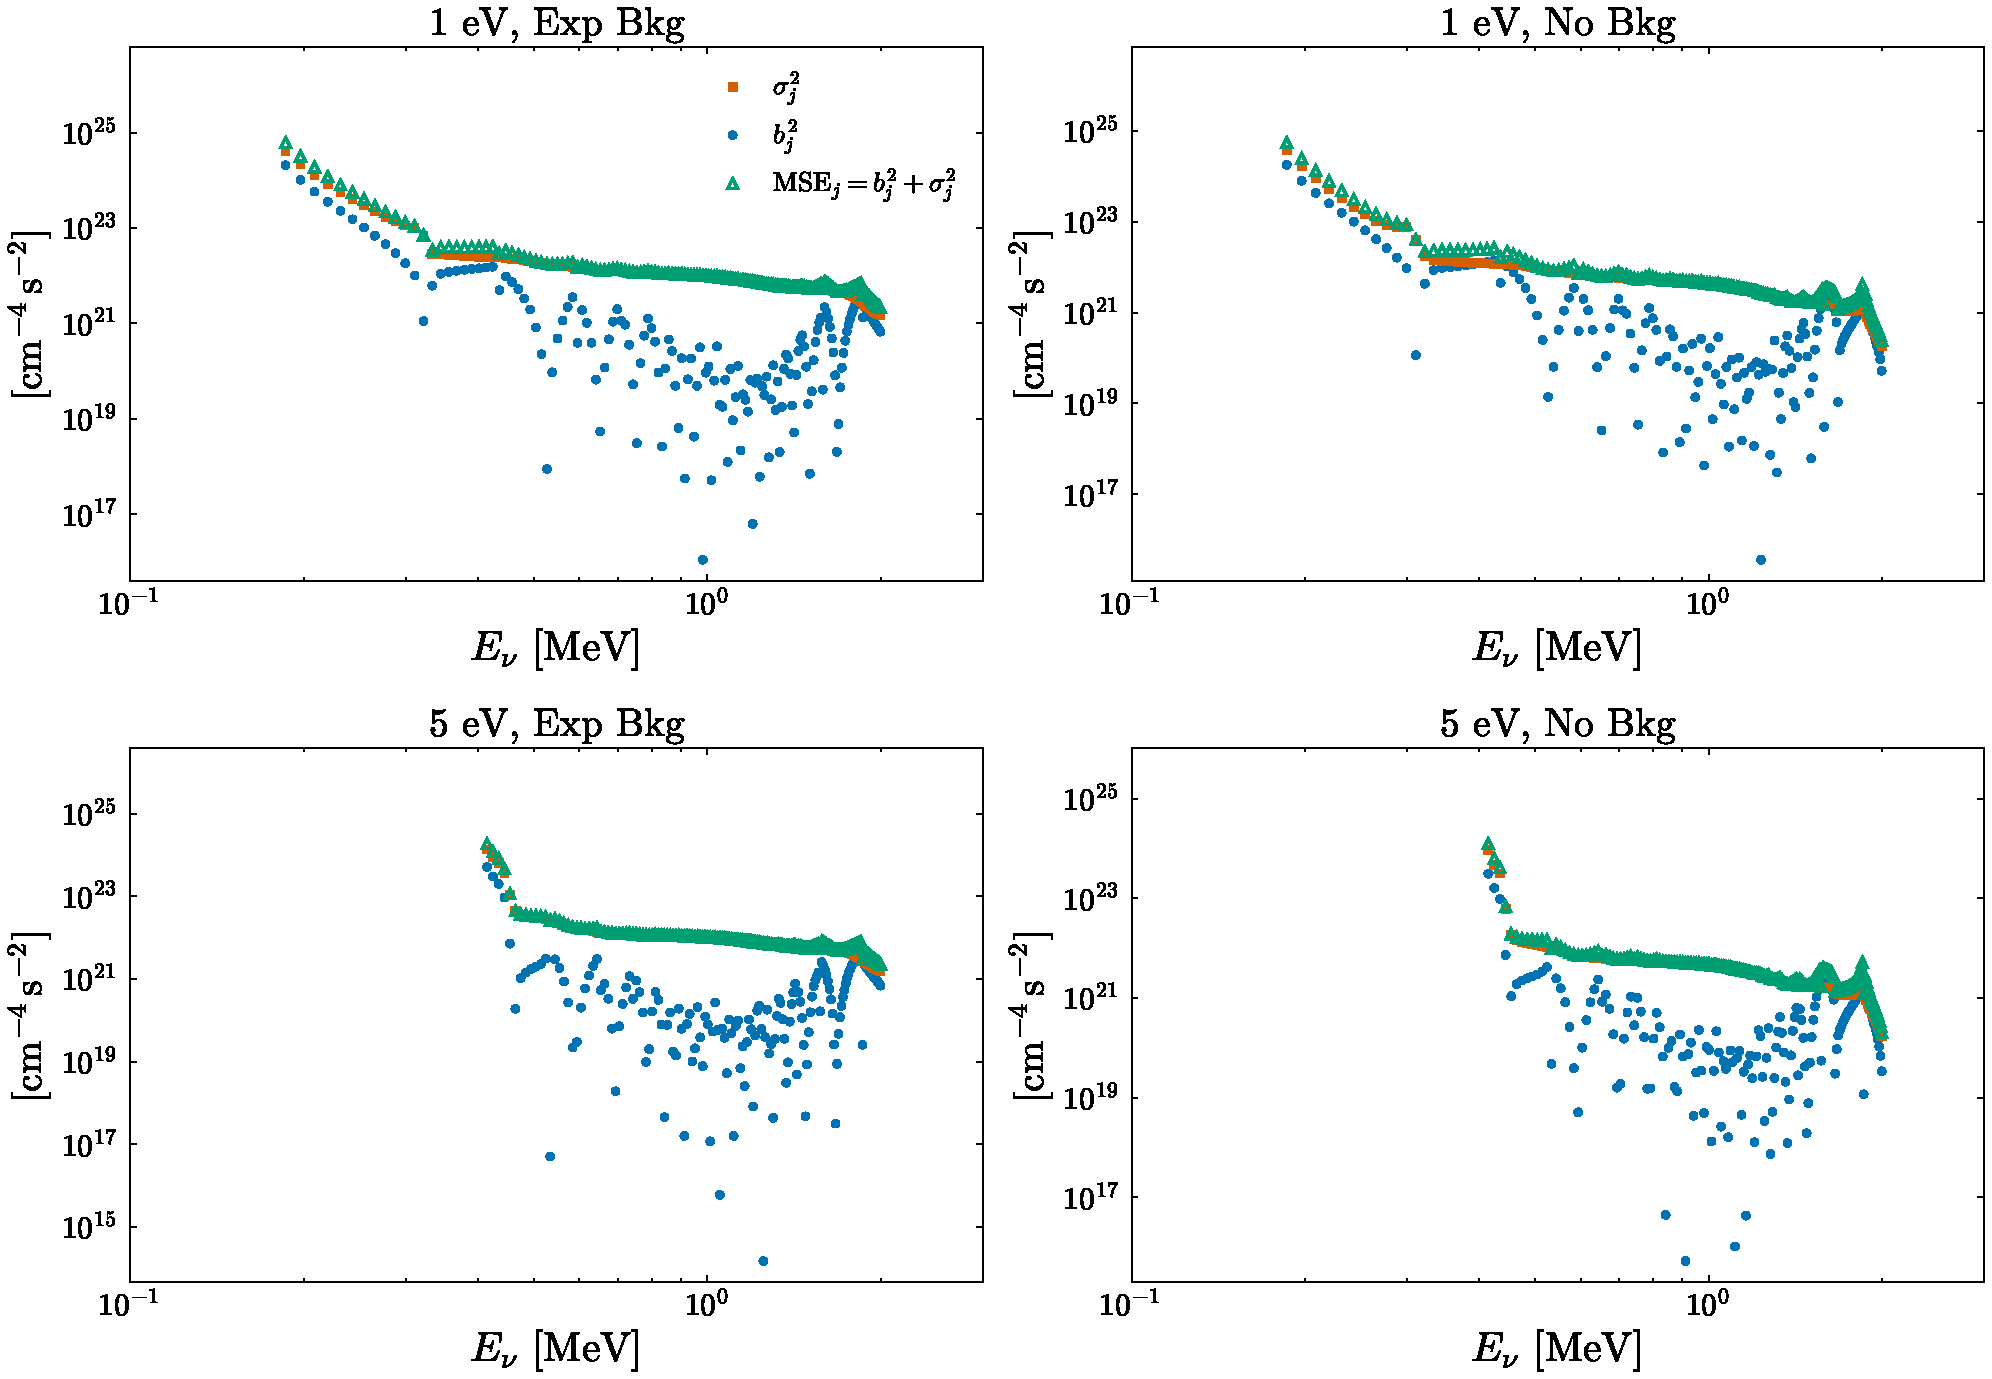
\includegraphics[width=\textwidth]{abs_b2_s2_mse_N160_M10000.pdf}
\caption{Squared bias $b_j^2$ (blue circles), variance $\sigma_j^2$
(orange squares), and ${\rm MSE}_j=b_j^2+\sigma_j^2$ (green open triangles)
of the unfolded $\delta\Phi_j$, in absolute units of integrated flux
squared, for the same four configurations and pseudo-experiment ensembles
as in Fig.~\ref{fig:relbiasdisp}.  The deep downward spikes of $b_j^2$
occur where the bias crosses zero.}
\label{fig:absmse}
\end{figure*}

% ---------- (A3) ratio b^2 / MSE ----------
\begin{figure*}[t]
\centering
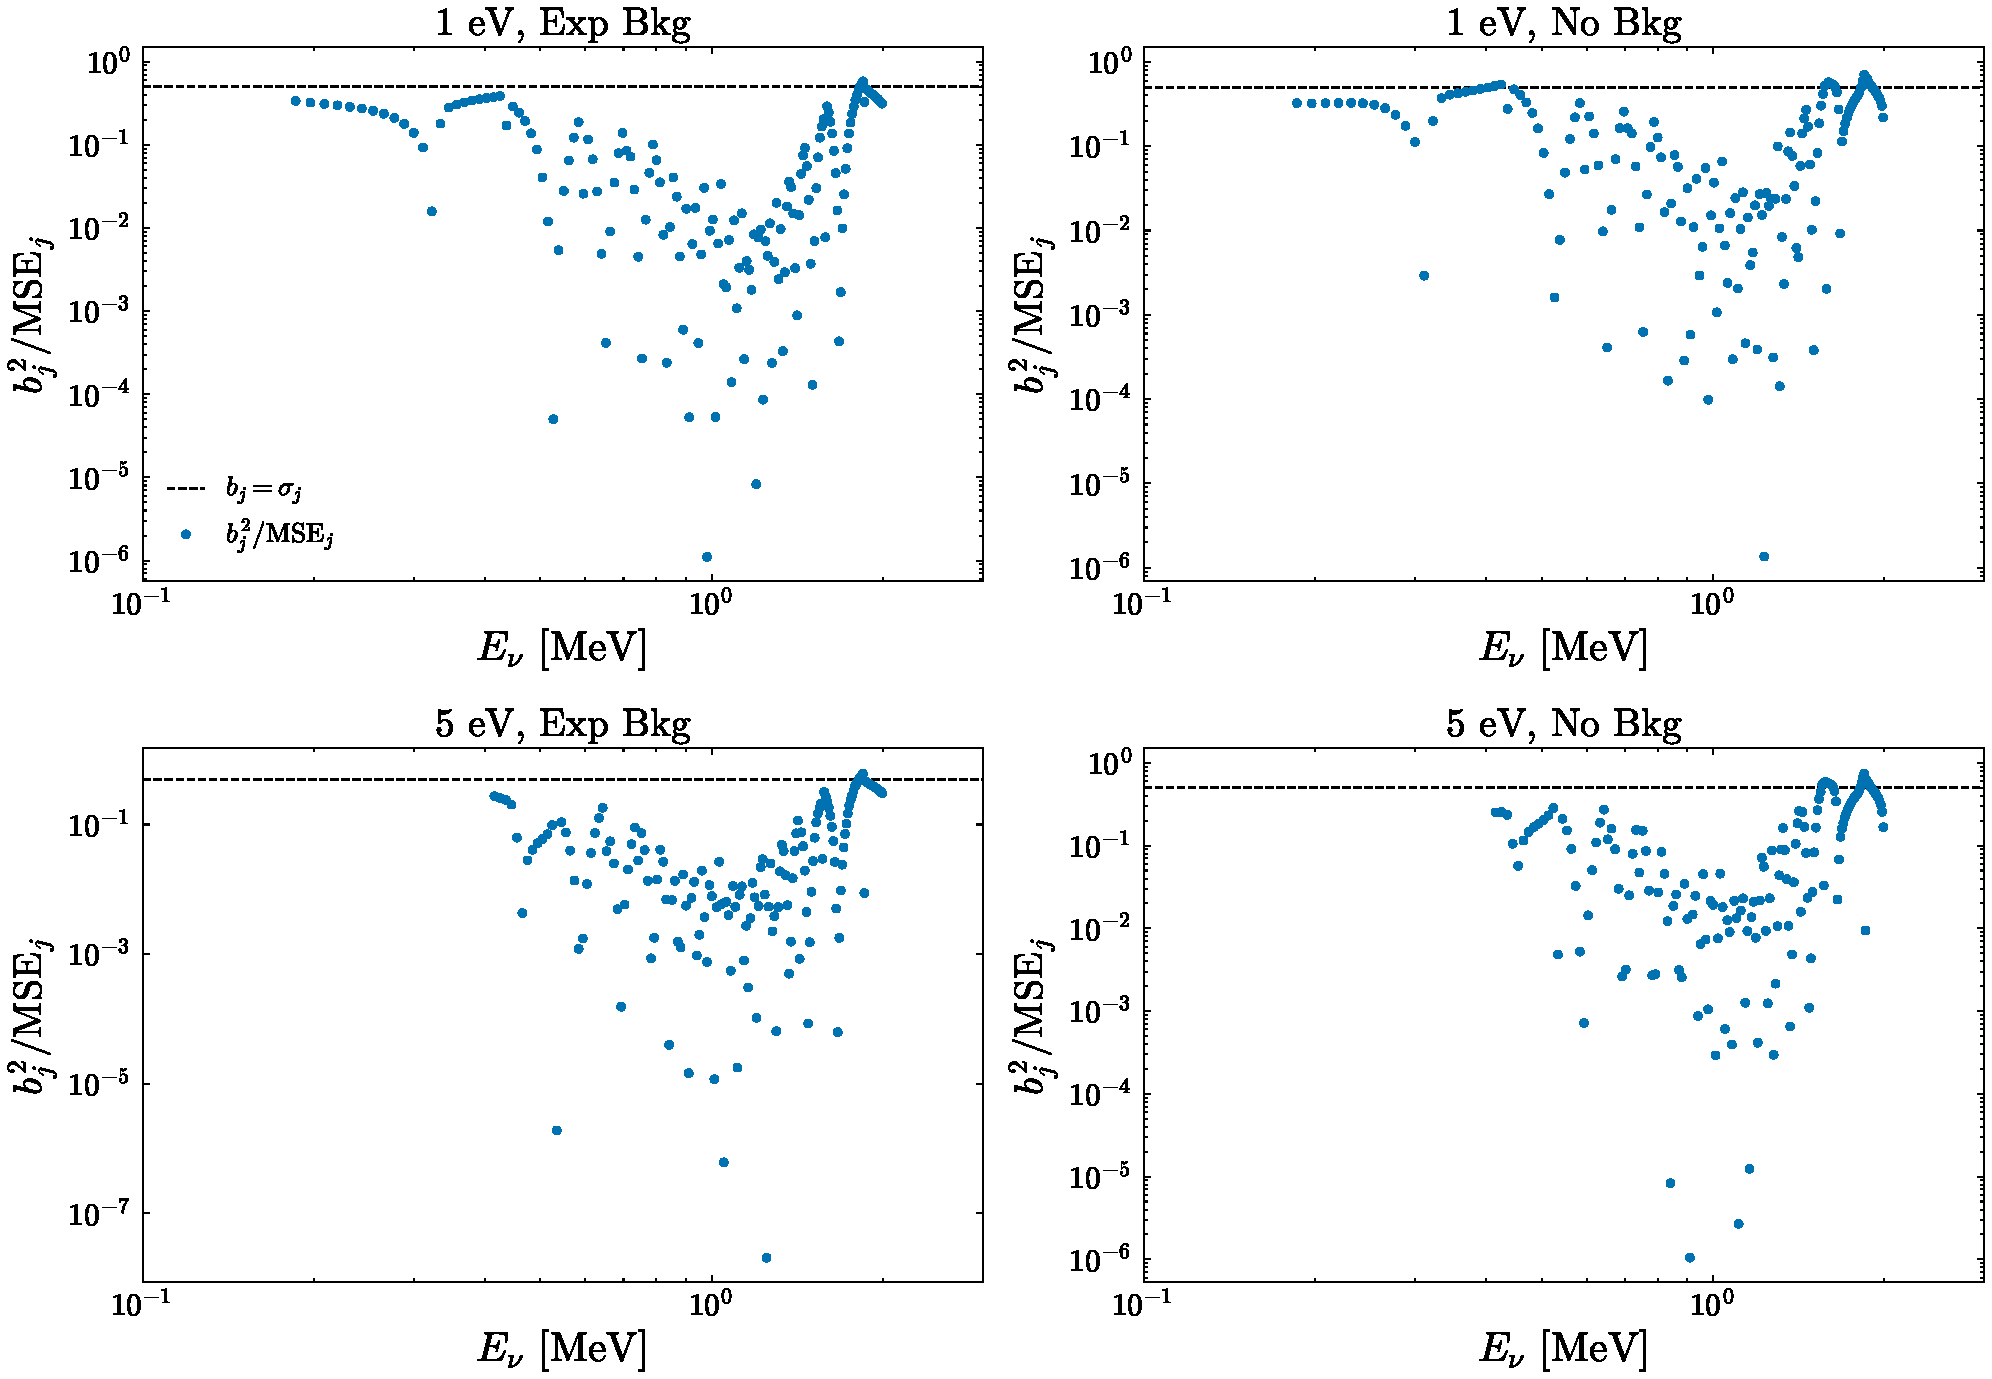
\includegraphics[width=\textwidth]{ratio_b2_over_mse_N160_M10000.pdf}
\caption{Ratio $b_j^2/{\rm MSE}_j$ for the same four configurations and
pseudo-experiment ensembles as in Fig.~\ref{fig:relbiasdisp}.  The dashed
line marks $b_j^2/{\rm MSE}_j=1/2$, i.e.\ $|b_j|=\sigma_j$.  Over most of
the energy range the ratio is below a few percent, so the MSE is dominated
by the variance; only in the lowest- and highest-energy intervals does the
bias contribute comparably to the dispersion.}
\label{fig:b2overmse}
\end{figure*}

% ============================================================
% (B) Appendix D -- brief description of the procedure
% ============================================================
\appendix
\section{Bias, dispersion, and mean squared error of the unfolded spectrum}
\label{app:biasprocedure}

To quantify the bias and the statistical dispersion of the unfolded
$\delta\Phi_j$ we use pseudo-experiments generated from the best fit
itself (a parametric bootstrap; see e.g.\ Ch.~11 of
Ref.~\cite{Cowan}), so that the input ``true'' spectrum is the best fit
$\delta\Phi_j^{\rm Best\ fit}$ to the simulated data, and all other inputs
are known exactly.

The procedure is as follows.
\begin{enumerate}
\item From the best fit, compute the expected total number of events in
each observed recoil-energy bin $i$, $N_i$, which includes the expected
signal produced by $\delta\Phi_j^{\rm Best\ fit}$ and the nominal
background $B_i$.
\item For each pseudo-experiment $m=1,\dots,M$, generate total observed
counts by fluctuating each bin independently with a Gaussian,
$n_i^{(m)}=N_i+\mathcal{N}(0,\sqrt{N_i})$, and an independent background
estimate $B_i^{(m)}=B_i+\mathcal{N}(0,\sqrt{B_i})$, which is subtracted in
the fit.  Only the total counts and the background estimate are
fluctuated, both with Gaussian distributions.  Since the difference of two
independent Gaussian variables is Gaussian, the effective signal
$n_i^{(m)}-B_i^{(m)}$ is also Gaussian distributed, as appropriate for a
counting experiment in the large-count regime.
\item Fit each pseudo-data set with exactly the same procedure used for
the simulated data (same response matrix, number of intervals
$N_{\rm int}$, shape constraints, and test statistic), obtaining
$\delta\hat\Phi_j^{(m)}$.
\item From the $M$ results compute, for each neutrino-energy interval $j$,
\begin{equation}
\overline{\delta\Phi}_j=\frac{1}{M}\sum_{m=1}^{M}\delta\hat\Phi_j^{(m)},
\qquad
b_j=\overline{\delta\Phi}_j-\delta\Phi_j^{\rm Best\ fit},
\end{equation}
\begin{equation}
\sigma_j^2=\frac{1}{M-1}\sum_{m=1}^{M}
\left(\delta\hat\Phi_j^{(m)}-\overline{\delta\Phi}_j\right)^{2},
\qquad
{\rm MSE}_j=b_j^2+\sigma_j^2 .
\end{equation}
\end{enumerate}

We use $M=10^4$ pseudo-experiments for each of the four configurations.
The Monte-Carlo uncertainty of the bias is
${\rm Err}(b_j)=\sigma_j/\sqrt{M}$, i.e.\ $1\%$ of $\sigma_j$, and that of
the variance is
${\rm Err}(\sigma_j^2)=\sigma_j^2\sqrt{2/(M-1)}\simeq1.4\%$.
The results are shown in
Figs.~\ref{fig:relbiasdisp}--\ref{fig:b2overmse}.
